

\section{harware}

Con el objetivo de detallar el hardware usado para la ejecucion del programa
se eneseña la salida por pantalla del comando "lscpu".



\begin{figure}[h p]
    \centering
    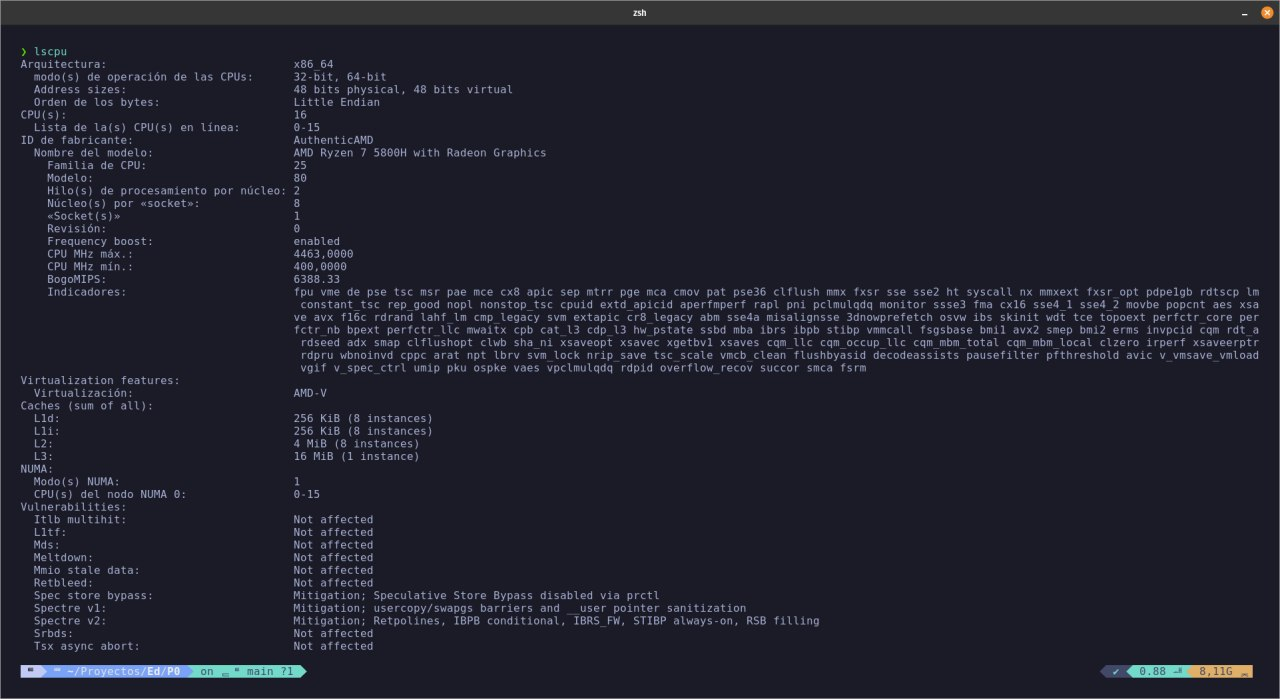
\includegraphics[clip,width=1.1\textwidth ]{archivos_auxiliares/lscpu.png}
    \caption{Comando lscpu}
    \label{lscpu_command}
\end{figure}

\section{software}

Con el objetivo de detallar el software usado para la ejecucion del programa 
se eneseña la salida por pantalla del programa "Neofetch":

\begin{figure}[h p]
    \centering
    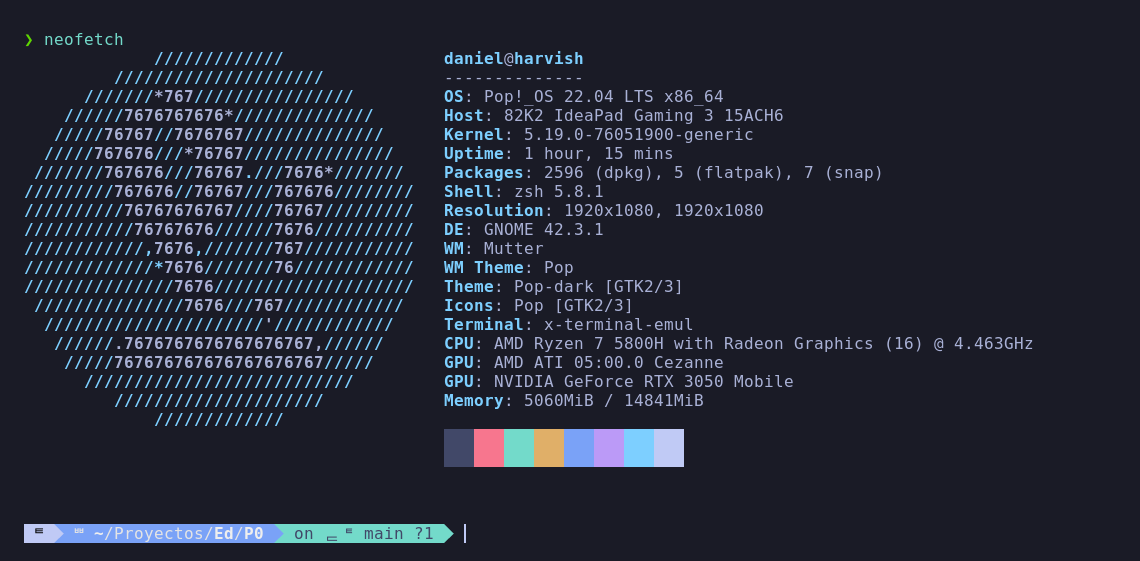
\includegraphics[clip, width=0.86\textwidth] {archivos_auxiliares/neofetch.png}
    \caption{Comando lscpu}
    \label{neofetch_command}
\end{figure}


A continuación se muestra la version del compilador c++ usado en este ejercicio:


\begin{figure}[h p]
    \centering
    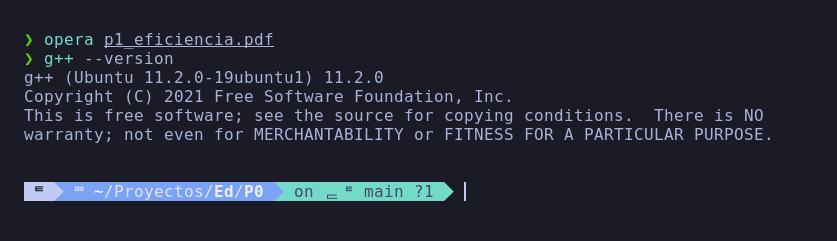
\includegraphics[width=1\textwidth]{archivos_auxiliares/g++.png}
    \caption{Comando lscpu}
    \label{g++_command}
\end{figure}

